\documentclass[journel,12pt,twocoloums]{IEEEtran}

\title{Assignment 8-Probability and Random Variable}
\author{Annu-EE21RESCH01010}
\date{13 January 2020}

\usepackage{amsthm}
\usepackage{graphicx}
\usepackage{mathrsfs}
\usepackage{txfonts}
\usepackage{stfloats}
\usepackage{pgfplots}
\usepackage{cite}
\usepackage{cases}
\usepackage{mathtools}
\usepackage{caption}
\usepackage{enumerate}	
\usepackage{enumitem}
\usepackage{amsmath}
\usepackage[utf8]{inputenc}
\usepackage[english]{babel}
\usepackage{multicol}
%\usepackage{xtab}
\usepackage{longtable}
\usepackage{multirow}
%\usepackage{algorithm}
%\usepackage{algpseudocode}
\usepackage{array,multirow}
\usepackage{enumitem}
\usepackage{mathtools}
\usepackage{gensymb}
\usepackage{hyperref}
%\usepackage[framemethod=tikz]{mdframed}
\usepackage{listings}
    %\usepackage[latin1]{inputenc}                                 %%
    \usepackage{color}                                            %%
    \usepackage{array}                                            %%
    \usepackage{longtable}                                        %%
    \usepackage{calc}                                             %%
    \usepackage{multirow}                                         %%
    \usepackage{hhline}                                           %%
    \usepackage{ifthen}                                         %%
  \providecommand{\nCr}[2]{\,^{#1}C_{#2}}
  \providecommand{\nPr}[2]{\,^{#1}P_{#2}}
  \lstset{
%language=C,
frame=single, 
breaklines=true,
columns=fullflexible
}

 \begin{document}
 \maketitle
\textbf{Download latex code from here-}\\
\begin{lstlisting}
 https://github.com/annu100/AI5002-Probability-and-Random-variables/tree/main.tex/ASSIGNMENT_8
 \end{lstlisting}
 \textbf{Download python code from here-}\\
\begin{lstlisting}
 https://github.com/annu100/AI5002-Probability-and-Random-variables/tree/main.py/ASSIGNMENT_8
 \end{lstlisting}
 \section{Problem Statement-Problem 3.7}


Let X represent the difference between the
number of heads and the number of tails
obtained when a coin is tossed 6 times. What
are possible values of X?
\section{Solution}
Let $X_1$ denotes the number of heads and $X_2$ denotes the number of tails that occur when a coin is tossed 6 times.\\

let n is total number of tosses and p is probability of getting head \\
p=q=0.5\\
Clearly, $X_1 \sim Bin(n=6,p)$\\
and $X_2 \sim Bin(n=6,1-p=q)$.\\
$\therefore n-X_2 \sim Bin(6, p)$.\\
By reproductive property,
\begin{align}
    X_1+n-X_2 \sim Bin(6+6, p)
\end{align}
$X=X_1-X_2$. 
\begin{align}
    P(X=x) = \binom{6+6}{6+x} p^{6+x} q^{6-x}, x= -6\ \text{to}\ 6 

    \therefore P(X=x) = \binom{12}{6+x}\brak{\frac{1}{2}}^{12},x= -6\ \text{to}\ 6 
\end{align}
 therefore,X can have any values between -6 to 6.
 

\section{Simulations}
Question-Plot the sum and difference of 2 bernaulli random variables\\
\subsection{Simulations-solutions}



\begin{figure}
\centering
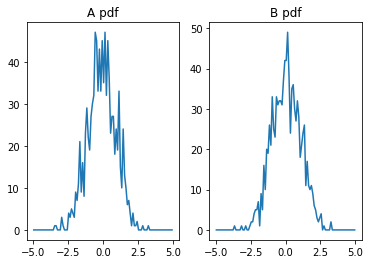
\includegraphics[width=\columnwidth] {pdf_A_B.png}
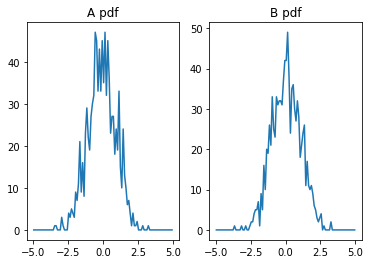
\includegraphics[width=\columnwidth] {pdf_sum.png}
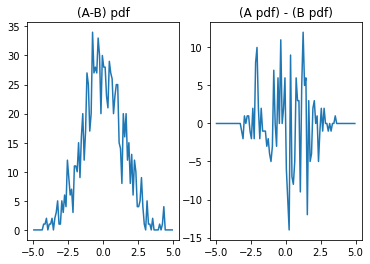
\includegraphics[width=\columnwidth] {pdf_subtract.png}
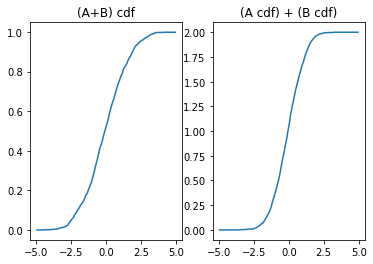
\includegraphics[width=\columnwidth] {cdf_sum.png}
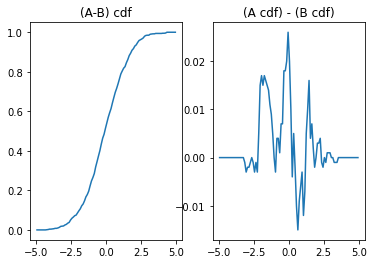
\includegraphics[width=\columnwidth] {cdf_subtract.png}
\end{figure}
\\
\\
\\

z=(x-$\mu$)/$\sigma$ \sim N(0,1)\\
where\\
$\mu$=n*p\\
and $\sigma$=\sqrt{n*p(1-p)}\\
\text{So,basically normal distributions are approximation of binomial distributions.}\\

PDF of 2 individual binomial random variables are plotted.\\

PDF of sum of 2 individual random variables and sum of their individual pdfs are plotted and compared.\\
PDF of difference of 2 individual random variables and difference of their individual pdfs are plotted and compared.\\
CDF of 2 individual binomial random variables are plotted.\\

CDF of sum of 2 individual random variables and sum of their individual Cdfs are plotted and compared.\\
CDF of difference of 2 individual random variables and difference of their individual cdfs are plotted and compared.\\
If x is a random variable with distribution Bin(n, p), then for sufficiently large n, the distribution of the variable.




\end{document}

        

